\section{Grundlagen und Begriffserklärungen}

\subsection{Die Composable-Enterprise-Architektur}

\subsubsection{Begriffserklärung und Abgrenzung}
\label{sec:CEA_B}
Flexibilität, Resilienz und Agilität. Nach Ansicht von Steve Denning, Managementberater und Autor der Forbes, stellen diese Eigenschaften wesentliche Faktoren dar, welcher zur Steigerung der Wettbewerbsfähigkeit von Unternehmen beitragen \cite{Denning.20170210}. Für Analystenhäuser wie Gartner steht dabei fest, dass es technologischer Innovation benötigt, um einhergehende Herausforderungen erfolgreich zu bewältigen und eine kontinuierliche Unternehmenstransformation voranzutreiben. Gartner empfiehlt dabei monolithische und starre Unternehmensarchitekturen, durch einen modularen Organisationsaufbau zu ersetzen. In seinen Veröffentlichungen verwendet Gartner für dieses Konzept den Begriff der \textbf{\ac{CEA}}.
\begin{center}
	\begin{figure}[H]
		\centering
		\scalebox{0.2}{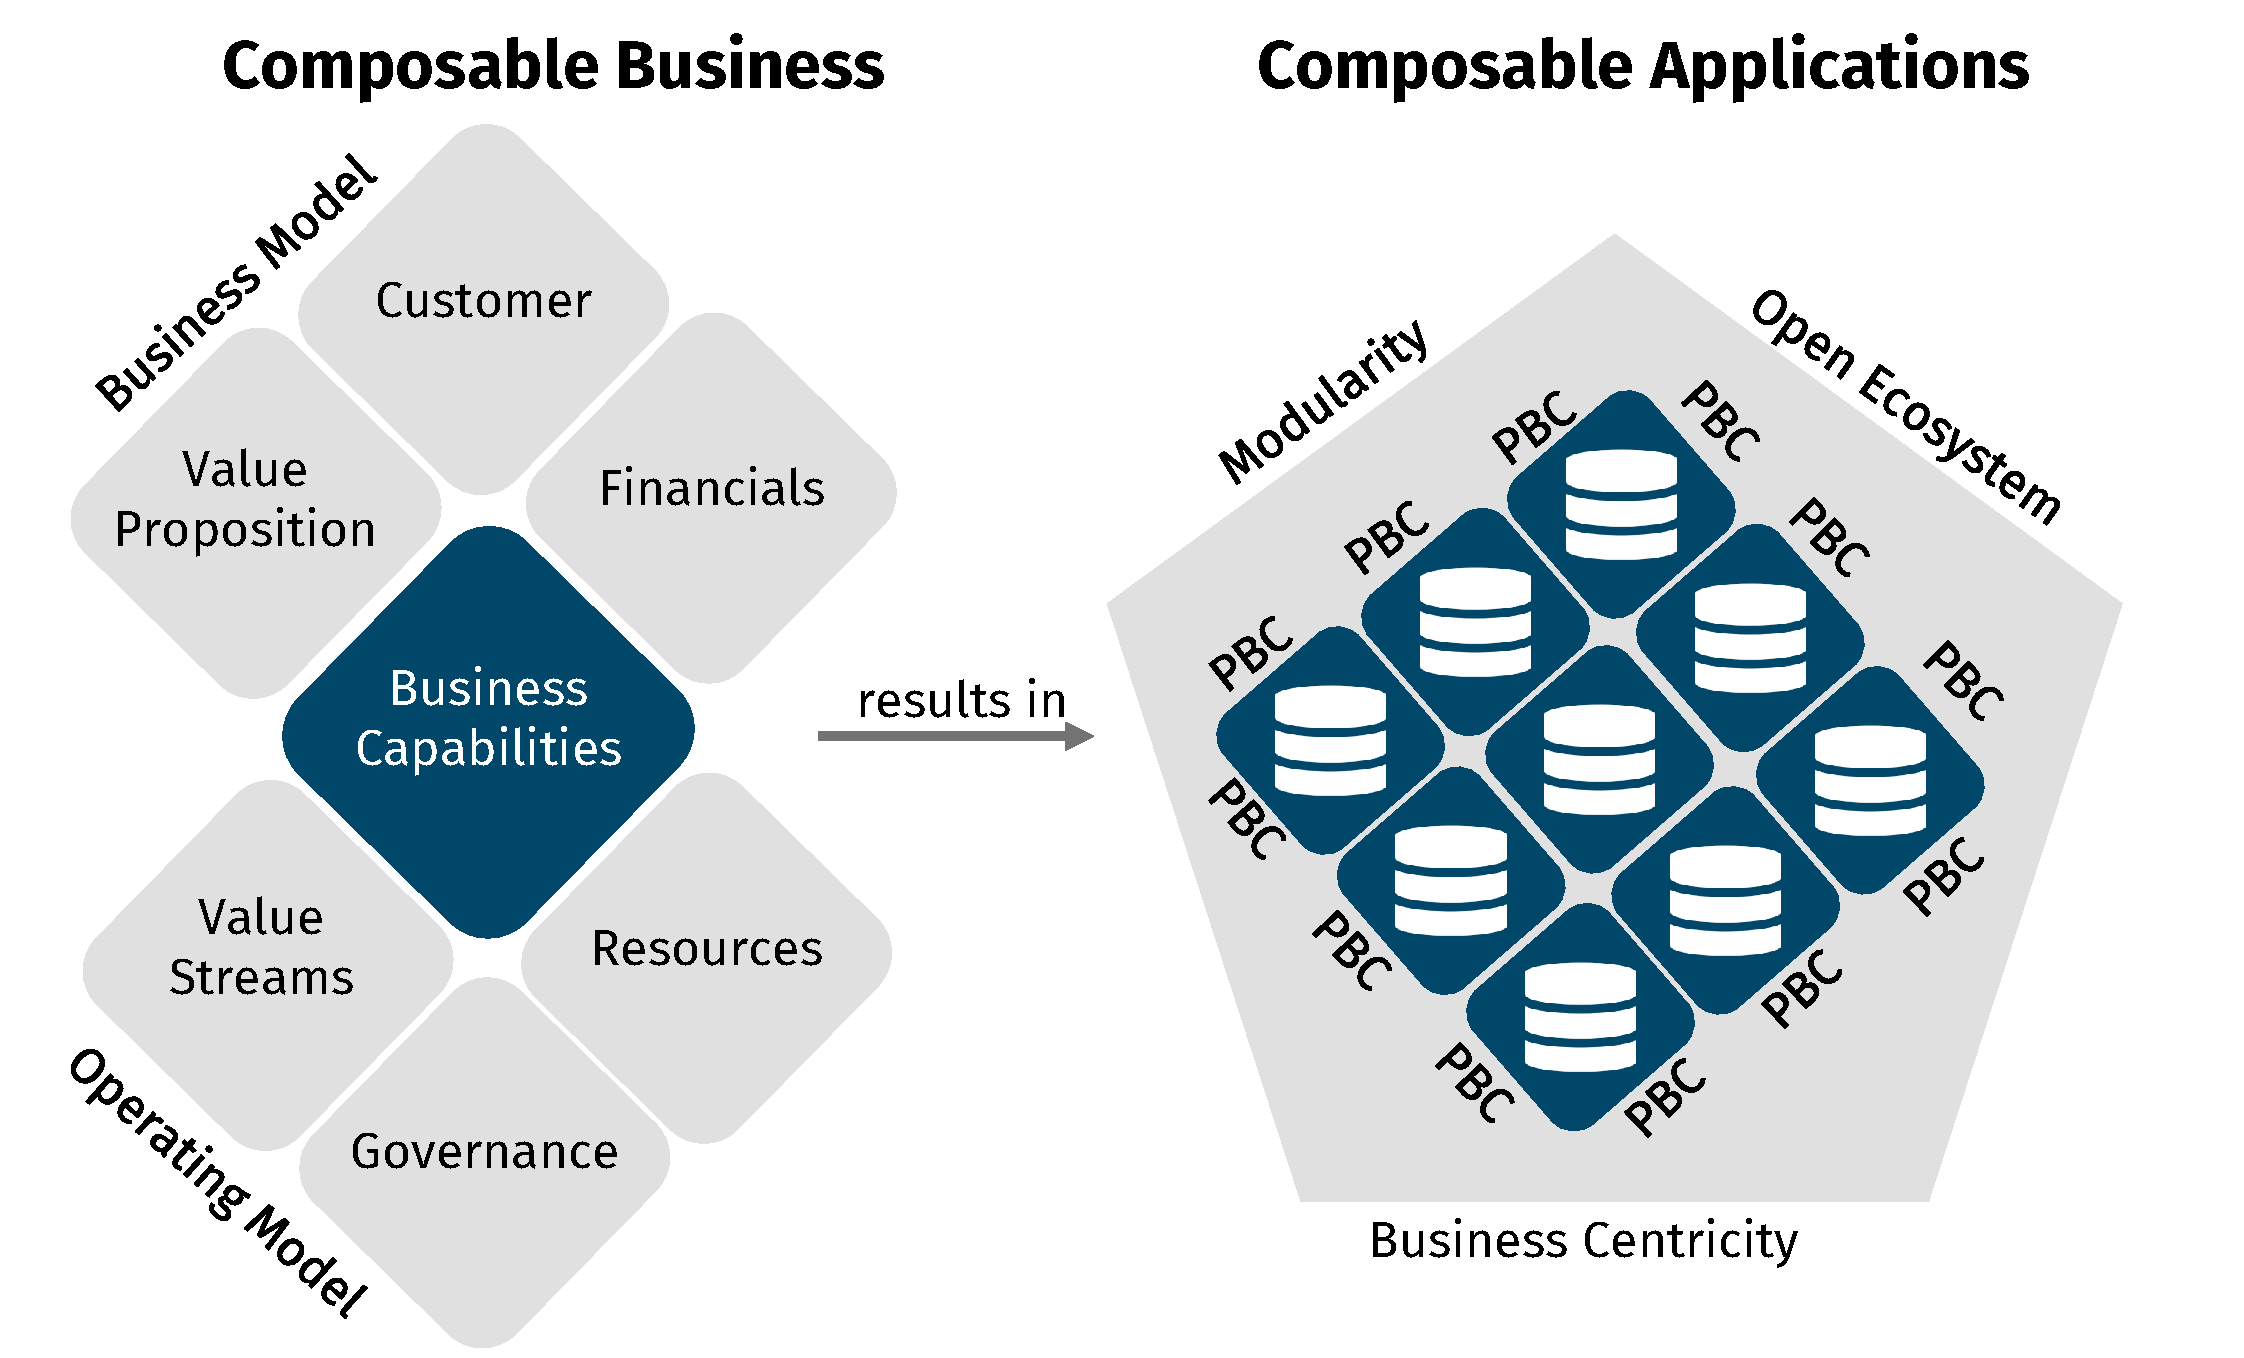
\includegraphics{CEA}}
		\caption[Entstehung einer Composable-Enterprise-Architektur]{Entstehung einer Composable-Enterprise-Architektur. In Anlehnung an Schönstein \cite{Schonenstein.20230103}.}
		\label{fig:CEA_S}
	\end{figure}	
\end{center}
\vspace*{-15mm}
In der Literatur wird die CEA dabei wie folgt definiert:\vspace{2mm}\\
\textit{\enquote{The Composable-Enterprise-Architecture is an architecture that delivers business outcomes and adapts to the pace of business change. It does this through the assembly and combination of packaged business capabilities \cite{.20230313}.}}\vspace{2mm}\\
Ein CE ist somit ein aus mehreren Bausteinen, sog. \textit{\ac{PBC}} bestehendes Unternehmen. PBCs sind vorgefertigte Softwareelemente, welche jeweils eine bestimmte Geschäftsfunktion abdecken (s. Abb. \ref{fig:CEA_S}). Das Konzept der PBCs fußt dabei auf den drei Prinzipien der CEA: \textit{Modulare Architektur}, \textit{Offenes Ökosystem} und \textit{Businesszentriertheit} \cite{.20230313}. Laut Gartner müssen Unternehmen nicht nur \enquote{akzeptieren, dass der disruptive Wandel zur Normalität gehört}. Vielmehr sollten diese den disruptiven Wandel als \enquote{Chance begreifen und ihn nutzen, um eine \textit{modulare Architektur} zu implementieren} \cite{.20230313}. In diesem Kontext wird von dem Analystenhaus Gartner ebenfalls der Begriff des \textit{Composable-Enterprise-Ressourcen-Planning-Systems (Composable-\acs{ERP}-Systems)} verwendet. Hierbei stellen die modularen Komponenten (PBCs) vorgefertigte Geschäftsfunktionen- bzw. prozesse dar, welche als Module in ein Composable-ERP-System integriert werden können. Diese PBCs können etwa Funktionen wie Finanzbuchhaltung, Einkauf, Verkauf, Lagerverwaltung, Produktion oder Personalmanagement enthalten. Ergibt sich eine Änderung in den Geschäftsanforderungen, ermöglicht diese Architektur ein flexibles und isoliertes Austauschen, Verändern sowie Weiterentwickeln einzelner PBCs \cite[315]{Chang.1019202010232020}. Durch die unabhängige Bereitstellung der Softwarekomponenten ist es weiterhin möglich, einzelne Module einer CEA skalierbar zu gestalten, ohne dabei die Gesamt-Suite anpassen zu müssen. Insbesondere für Start-ups ist dieser Vorteil von hoher Bedeutung, da diese somit in der Lage sind, Unternehmenssoftware flexibel an wachsenden Geschäftsanforderungen anzupassen.  
\begin{center}
	\begin{figure}[H]
		\centering
		\scalebox{0.30}{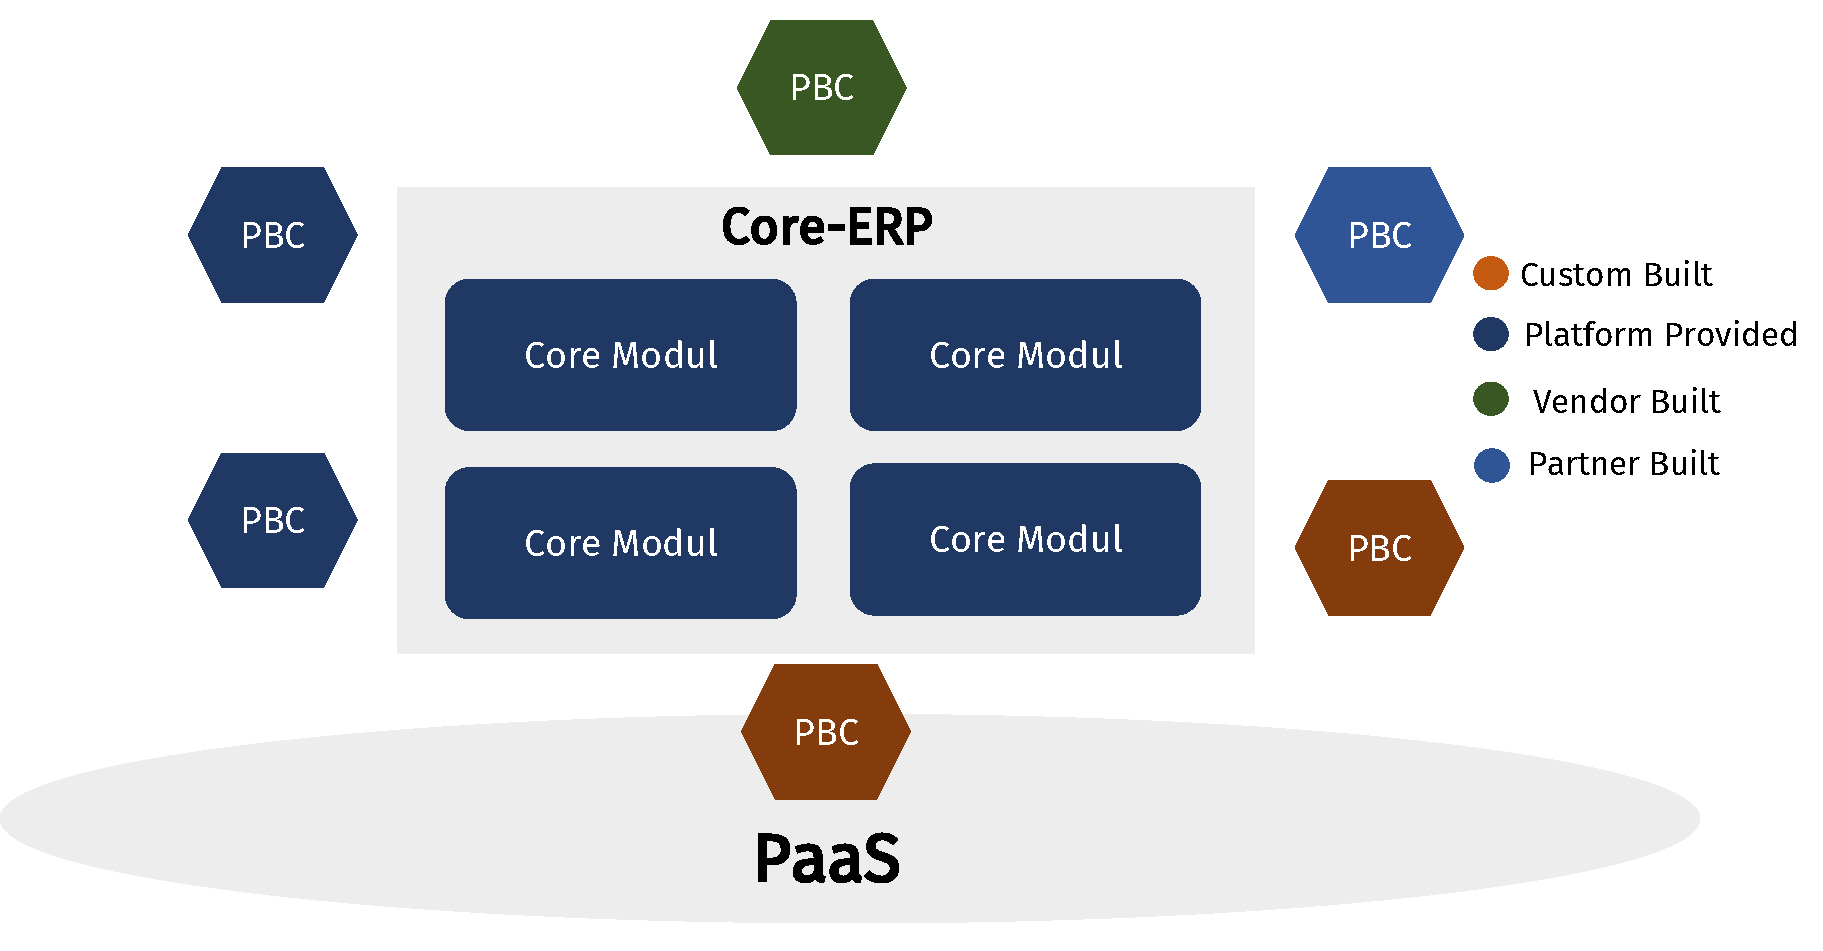
\includegraphics{CERP}}
		\caption[Bestandteile eines Composable-ERP-Systems]{Bestandteile eines Composable-ERP-Systems. Eigene Darstellung.}
		\label{fig:CERP}
	\end{figure}	
\end{center}
\vspace*{-15mm}
Ein Composable-ERP-System verfügt über eine Kollektion von Kernkomponenten (s. Abb. \ref{fig:CERP})\cite[7]{Sensedia.2020}. Diese Kernkomponenten werden i.d.R. von einem einzigen ERP-Anbieter bereitgestellt und können deshalb ohne hohen Aufwand integriert und aufeinander abgestimmt werden \cite[S. 29 ff.]{Sarferaz.2022}. Bei diesen Komponenten handelt es sich dabei um Funktionalitäten, welche das Hauptgeschäft eines Unternehmens unterstützen. Um den sich ändernden Geschäftsanforderungen gerecht zu werden, können diese Kernkomponenten durch zusätzliche PBCs erweitert werden \cite[58]{.2009}. Dieses Konzept basiert auf dem Prinzip des \textit{offenen Ökosystems}. Die externen, in das Kern-ERP-System integrierbaren PBCs, umfassen dabei i.d.R. stark spezialisierte Funktionalitäten. So könnte sich ein E-Commerce-Unternehmen dazu entschließen, eine Kern-\acl{CRM}-Komponente (Kern-CRM-Komponenten) um eine KI-basierte Kundenanalysefunktion zu erweitern. Um die Integration dieser modularen Komponenten zu erleichtern, stellen ERP-Anbieter auf ihren Cloud-Plattformen einen zur Bündelung der PBCs verwendeten Marktplatz zur Verfügung. Die dabei angeboten Komponenten können zusätzliche Funktionen des ERP-Kern\-anbieters oder externe Komponenten von Spezialherstellern darstellen. Auf diese Weise haben Mitarbeiter oder Teams die Möglichkeit, innerhalb ihres Unternehmens auf diesen Marktplatz zuzugreifen und Werkzeuge (PBCs), welche zur Unterstützung der operativen Tätigkeiten benötigt werden, ohne hohen Aufwand zu aktivieren. Das ERP-System kann somit auf die spezifischen Bedürfnisse und Anforderungen der Unternehmen zugeschnitten werden \cite[S. 29 ff.]{Sarferaz.2022}. IT-Systeme dienen dem Zweck der Unterstützung operativer Aufgaben. Um eine anwenderzentrierte Gestaltung der auf dem Marktplatz angebotenen Werkzeuge zu ermöglichen, sollte der Fokus dieser Tools auf den Bedürfnissen und Erwartungen der Anwender liegen (\textit{Businesszentriertheit}). Deshalb ist essenziell, dass Mitarbeiter Systeme intuitiv nutzen und ggf. weiterentwickeln und anpassen können, ohne dabei von IT-Abteilungen abhängig zu sein \cite{.20230313}. Dabei soll die Verwendung von Low-Code/No-Code-Plattformen Abhilfe schaffen. Diese ermöglichen den Mitarbeiter eigene PBCs zu entwickeln ohne auf spezielle IT-Kenntnisse oder -Ressourcen angewiesen zu sein. Damit wird die Agilität und Flexibilität der CEs erhöht, während die Abhängigkeit von IT-Abteilungen reduziert wird.

\subsubsection{Technologische Konzepte des Composable-Enterprises}
Um die in Kapitel \ref{sec:CEA_B} aufgeführten betriebswirtschaftlichen Grundsätze in das Unternehmen zu integrieren, benötigt es verschiedener technologischer Konzepte. Zusammenfassen lassen sich diese mit dem Akronym \textit{MACH}: \textit{\acl{MACH}}.
\begin{center}
	\begin{figure}[H]
		\centering
		\scalebox{0.3}{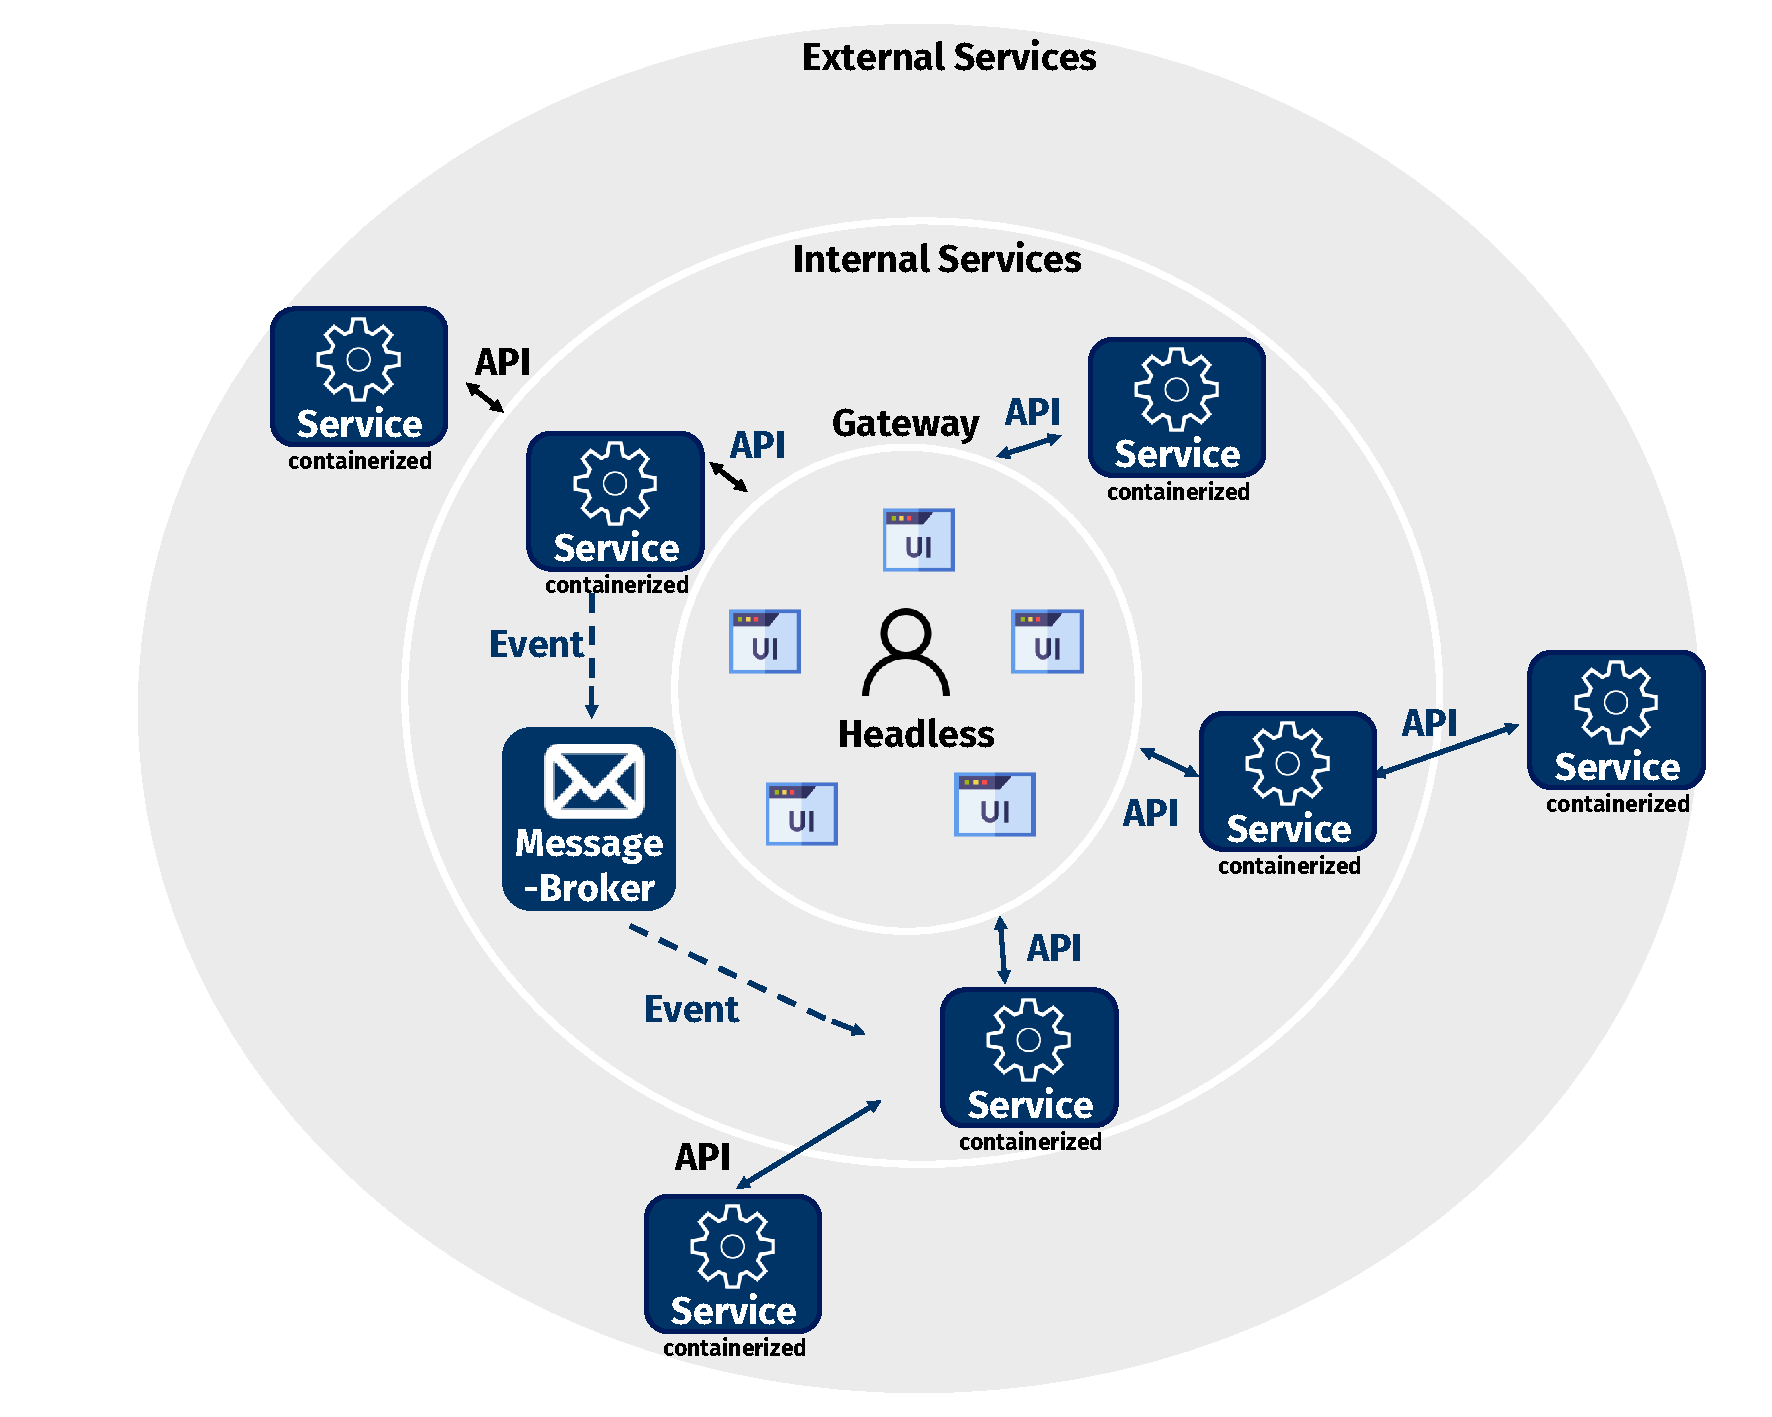
\includegraphics{CEA_K}}
		\caption[Technische Realisierung der Composable-Enterprise-Architektur]{Technische Realisierung der Composable-Enterprise-Architektur. Eigene Darstellung.}
		\label{fig:CEA_K}
	\end{figure}	
\end{center}
\vspace*{-15mm}
Der zentrale Einstiegspunkt in eine CE-Anwendung ist das User-Interface. Insbesondere für Content-Management-Systeme wird für Frontend-Entwicklungen das \textit{Headless-Konzept} verwendet (s. Abb. \ref{fig:CEA_K}). Dieses beschreibt, dass zwischen Front- und Backend keine feste Kopplung besteht. Vielmehr werden auf dem Backend standardisierte Daten verwaltet, welche auf verschiedenen Frontends ausgegeben werden können \cite{.20230313}. Die Geschäftsfunktionen einer CEA werden in verschiedene PBCs gekapselt. In der Applikationslogik des Backends kann ein PBC durch ein oder mehrere \textit{Microservices} dargestellt werden. Ein Microservice ist eine eigenständige Einheit, welche für eine spezifische Funktion zuständig ist. Im Kontext eines E-Commerce-Unternehmens könnte ein PBC etwa eine Bestellverwaltung sein. Diese Bestellverwaltung kann dabei aus verschiedenen Microservices, wie einem Bestellannahme-, Auftragsabwicklungs- oder Rechnungstellungsdienst bestehen. Microservices spielen dabei hauptsächlich für die technische Realisierung eine Rolle. Folglich sind diese für den Endanwender nicht erkennbar. Es ist möglich für jeden Service eine unterschiedliche Programmiersprache sowie Datenbank zu verwenden. So können Architektur und Technologien eines Dienstes unmittelbar an dessen betriebswirtschaftliche Anforderungen angepasst werden \cite[41]{.2009}. Zur Kommunikation zwischen Services werden standardisierte Schnittstellen, sog. \textit{\ac*{APIs}} verwendet. Mit APIs werden die von den Services bereitgestellten Funktionalitäten und Daten veröffentlicht \cite[15]{Biehl.2015}. Diese Schnittstellen können dabei unmittelbar von dem Frontend oder anderen Microservices konsumiert werden. Ein weiteres in CEs verwendetes Kommunikationskonzept ist die \textit{\ac{EDA}}. Die EDA ist ein Architekturkonzept, bei welchen Microservices asynchron über eine zentrale Vermittlungsinstanz, dem \textit{Message Broker}, kommunizieren \cite[54]{Bruns.2010}. Alle Komponenten der CEA werden auf einer Cloud-Plattform betrieben (\textit{Cloud-native}). Cloud-Computing ist ein Dienstleistungsmodell, welches Nutzern ermöglicht Ressourcen, wie Speicher, Analyse-Tools oder Software über das Internet von einem Cloud-Anbieter zu beziehen \cite[5]{Reinheimer.2018}. Dieses Computing-Modell ermöglicht IT-Services schnell und kosteneffizient an aktuelle Markterfordernisse anzupassen. Aufgrund der nutzungsabhängigen Bepreisung von Cloud-Plattformen können Dienste ohne hohen Investitionseinsatz auf- und abgebaut werden \cite[10]{Reinheimer.2018}. Für das Cloud-Computing werden durch das \ac{NIST} verschiedene Servicemodelle definiert. Neben \textit{\ac{SaaS}} und \textit{\ac{IaaS}}, bei welchem  eine Anwendung bzw. eine gesamte Infrastruktur in der Cloud gemietet wird, gibt es ebenfalls das \textit{\ac{PaaS}} \cite{Reinheimer.2018} \cite[9]{Reinheimer.2018}. Bei diesem Computing-Modell wird eine Plattform bereitgestellt, auf welcher Kunden eigene Anwendungen entwickeln, testen und betreiben können. Ein auf dieser Service-Ebene von der SAP bereitgestelltes Produkt ist die \ac{SAP BTP}. Diese stellt eine Reihe von Diensten und Funktionen zur Verfügung, mit welchen Unternehmen SAP-ERP-Systeme anpassen, integrieren und erweitern können. 

\subsection{Integration und Bereitstellung einer Cloud-Anwendung}
\subsubsection{Agile und DevOps als moderne Softwareentwicklungskonzepte}
Das Hauptaugenmerk eines CEs besteht darin, eine möglichst modulare und flexible Systemarchitektur zu schaffen. Damit soll sichergestellt werden, dass IT-Leistungen in einem sich stetig ändernden Umfeld schnell und risikoarm bereitgestellt werden. Das traditionelle Wasserfallmodell, welches eine sequenzielle Abfolge der Projektelemente \textit{Anforderung}, \textit{Design}, \textit{Implementierung}, \textit{Test} und \textit{Betrieb} vorgibt, besitzt dabei signifikante Limitationen. Die in dieser Methodik detailliert durchgeführte Vorabplanung, kann insbesondere in umfangreichen Langzeitvorhaben aufgrund unvorhersehbarer Externalitäten selten eingehalten werden \cite[5]{Vivenzio.2013}. Dies resultiert nicht nur in einem Anstieg der Kosten, sondern führt ebenfalls dazu, dass IT-Projekte länger als geplant ausfallen \cite[41]{Vieweg.2015}. Als Reaktion haben sich innerhalb der Projektmanagementlandschaft zunehmend \textbf{agile Vorgehensmodelle} etabliert.
Im Gegensatz zum Wasserfallmodell, welches eine umfassende Vorabplanung vorsieht, wird das Vorhaben in einer agilen Entwicklung in viele zyklische Einheiten, sog. \textit{Sprints}, segmentiert (s. Abb. \ref{fig:Agile_Cycle}) \cite[87]{Goll.2015}. Alle innerhalb des Projektumfangs zu entwickelnden Funktionalitäten werden dabei in einem zentralen Artefakt (\textit{Product Backlog}) festgehalten und von dem Produktverantwortlichen (\textit{Product Owner}) priorisiert. 
\begin{center}
	\begin{figure}[H]
		\centering
		\scalebox{0.5}{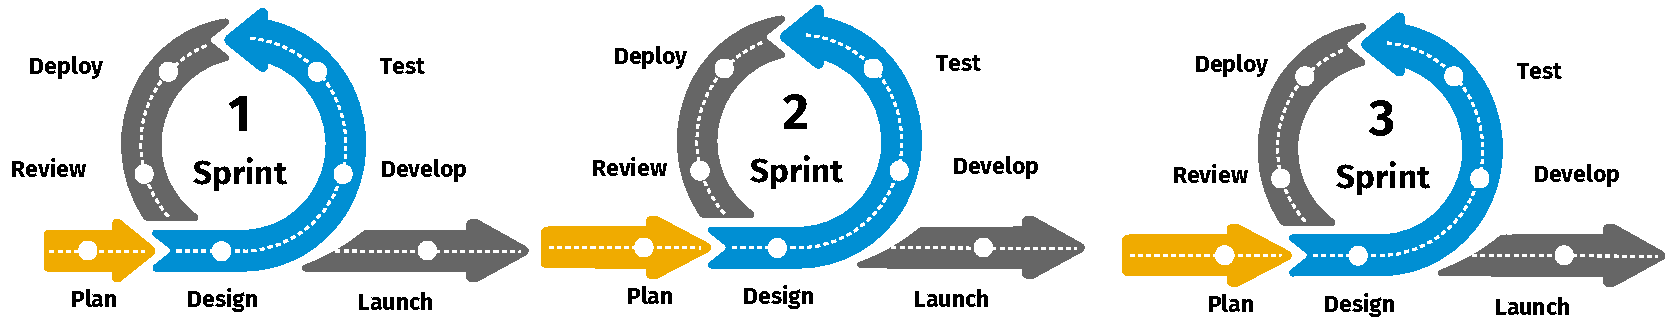
\includegraphics{Agile_Cycle}}
		\caption[Exemplarische Abfolge eines agilen Entwicklungszykluses]{Exemplarische Abfolge eines agilen Entwicklungszykluses. In Anlehnung an K\&C \cite{K&C.2021}.}
		\label{fig:Agile_Cycle}
	\end{figure}	
\end{center}
\vspace*{-15mm}
Sprints sind Durchläufe, welche i.d.R. einen Zeitraum von ein bis vier Wochen umfassen. Während dieses Abschnitts ist die Fertigstellung eines vor dem Sprint definierten Aufgabenkontingents (\textit{Sprint Backlog}) vorgesehen. Nach Abschluss eines Sprints soll dabei ein potenziell an den Kunden auslieferbares Produkt zur Verfügung gestellt werden. Dies erlaubt eine schnelle Bereitstellung funktionsfähiger Software. Nach Ablauf eines Sprints kann das an die Stakeholder ausgelieferte Artefakt als Feedback-Grundlage verwendet und im unmittelbaren Folge-Sprint eingearbeitet werden \cite[39]{K&C.2021}.
Innerhalb der letzten Dekade haben sich diverse auf agilen Prinzipien basierenden Vorgehensmodelle, wie Scrum, Kanban oder \ac{XP} in der Softwareentwicklung etabliert. Obwohl einige dieser Methoden zur erfolgreichen Zusammenarbeit innerhalb der Entwicklungsteams beigetragen haben, bleibt das sog.  \textit{Problem der letzten Meile} bestehen \cite{Qentelli.20230305}. Traditionell erfolgt eine funktionale Trennung der Entwickler- und IT-Betriebler-Teams. Das Problem der letzten Meile beschreibt dabei, dass aufgrund ausbleibender Kooperation dieser Teams der Programmcode nicht auf die Produktivumgebung abgestimmt ist. Erkenntnisse aus der Praxis zeigen, dass solche organisatorischen Silos häufig in einer schlechten Software-Qualität und somit in einem geminderten Ertragspotenzial bzw. in einer Erhöhung der Betriebskosten resultieren \cite[1]{Halstenberg.2020}. So geht aus der von McKinsey veröffentlichten Studie \textit{The Business Value of Design 2019} hervor, dass durchschnittlich 80 Prozent des Unternehmens-IT-Budgets zur Erhaltung des Status quo, also zum Betrieb bestehender Anwendungen verwendet wird. Stattdessen fordert das Beratungshaus eine Rationalisierung der Bereitstellung von Software, um finanzielle Mittel für wertschöpfende Investitionen zu maximieren \cite{.20230305}. Abhilfe schaffen kann das in der Literatur als \textbf{\ac{DevOps}} bekannte Aufbrechen organisatorischer Silos zwischen Entwicklung und dem IT-Betrieb \cite[1]{Halstenberg.2020}. 
Dabei stellt DevOps keine neue Erfindung dar. Stattdessen werden einzelne bereits bewährte Werkzeuge, Praktiken und Methoden, wie z.B. die agile Softwareentwicklung, zu einem umfassenden Rahmenwerk konsolidiert. Prägnant zusammenfassen lässt sich das DevOps-Konzept durch das Akronym CAMS: \textit{Culture (Kultur)}, \textit{Automation (Automatisierung)} und \textit{Measurement (Messung)} \cite[5]{Halstenberg.2020}. Dabei gilt \textit{Kultur} als das wohl wesentlichste DevOps-Erfolgselement. Diese bezweckt eine Kollaborationsmentalität, welche sich über alle Ebenen eines Unternehmens erstreckt. Operative Entscheidungen sollen dabei auf die Fachebenen herunter delegiert werden, welche aufgrund ihrer spezifischen Expertise am geeignetsten sind, Dispositionen zu verabschieden \cite[5]{Halstenberg.2020}. Eine \textit{Automatisierung} der Softwarebereitstellungsprozesse ermöglicht, sich wiederholende manuelle Arbeit zu eliminieren. Dies kann ebenfalls zur Rationalisierung und damit zur Senkung der IT-Betriebskosten beitragen. Der dabei erzielte Einfluss wird anhand verschiedener DevOps-Kennzahlen bemessen (\textit{Messung}). Neben der Systemverfügbarkeit und der Instandsetzungszeit ist für Softwareentwicklungsunternehmen insbesondere der \textit{Time-to-Market (\acs{TTM})} signifikant \cite[7]{Halstenberg.2020}. Dieser beschreibt die Zeitspanne zwischen Entwicklungsentstehungsprozess und der Markteinführung von IT-Services \cite[141]{Vesey.1992}. Dabei soll die mit DevOps angestrebte Verschmelzung der Entwicklungs- und Betriebsteams, die Automatisierung von Prozessen sowie die kontinuierliche Integration und Bereitstellung zu einer erheblichen Reduzierung dieser Metrik führen. Adam Caplan, leitender Strategieberater bei Salesforce, sieht in einer schnellen Bereitstellung von IT-Services angesichts der bei Softwareintegration entstehenden Komplexität, einen erheblichen Vorteil. So können Anwendungen schnellst möglichst in produktionsähnlichen Umgebungen getestet und sukzessive mit dem Kunden verbessert werden \cite{Vesey.1992}. 

\subsubsection{Automatisierung der Integrations- und Bereitstellungsprozesse}
\label{sec:CICD}
 Ein integraler Bestandteil des DevOps-Rahmen\-werks ist \textit{\ac{CI/CD}}. CI/CD ist ein Verfahren, welches zur Verbesserung der Qualität bzw. zur Senkung der Entwicklungszeit von IT-Services beiträgt. Abhilfe schaffen soll dabei eine sog. CI/CD-Pipeline, welche alle Schritte von Code-Integration bis Bereitstellung der Software automatisiert. Hauptaugenmerk liegt dabei auf einer zuverlässigen und kontinuierlichen Bereitstellung von Software \cite[471]{Zampetti.92720211012021}.
\begin{center}
	\begin{figure}[H]
		\centering
		\scalebox{0.4}{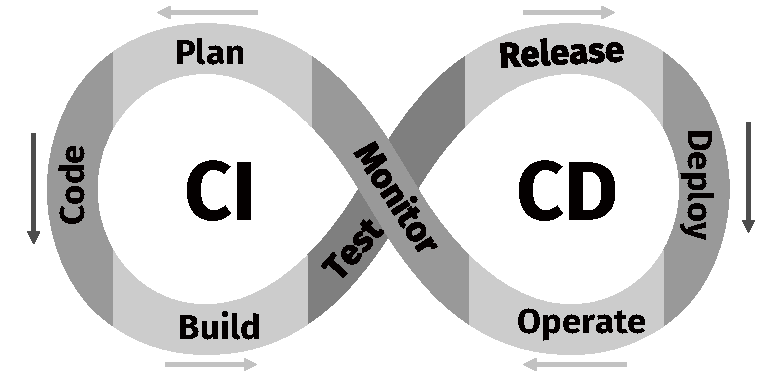
\includegraphics{CICD_Cycle}}
		\captionsetup{format=myformat}
		\caption[Aktivitäten im CI/CD-Prozess]{Aktivitäten im CI/CD-Prozess. In Anlehnung an Synopsys \cite{.20230201}.}
		\label{fig:CICD_Cycle}
	\end{figure}
\end{center}
\vspace*{-15mm}
Alle in diesem Prozess anfallenden Aktivitäten werden dabei im CI/CD-Zyklus der Abb. \ref{fig:CICD_Cycle} dargestellt. Der \acs{CI}-Prozess (Continuous-Integration-Prozess) bezweckt, dass lokale Quellcode\-änderungen in kurzen Intervallen und so schnell wie möglich in eine zentrale Codebasis geladen werden. Das frühzeitige Integrieren von Code soll dabei zu einer unmittelbaren und zuverlässigen Fehlererkennung innerhalb des Entwicklungsvorhabens beitragen \cite[471]{Zampetti.92720211012021}. 
Der erste Schritt des CI-Prozesses umfasst die Planung zu entwickelnder Services (\textit{Plan}: s. Abb. \ref{fig:CICD_Cycle}). Dabei soll festgestellt werden, welche Anforderungen eine Lösung besitzt bzw. welche Softwarearchitekturen sowie Sicherheitsmaßnahmen implementiert werden sollten. Um sicherzustellen, dass die in der Planung entworfene Anwendungsarchitektur auf das Design des Produktivsystems abgestimmt ist, sollte zu jedem Zeitpunkt das Know-how der Betriebsteams einbezogen werden \cite[16]{Halstenberg.2020}. Nach erfolgreichem Entwurf zu implementierender Anwendungs-Features beginnt die Entwicklung der IT-Services (\textit{Code}: s. Abb. \ref{fig:CICD_Cycle}). Arbeiten hierbei mehrere Entwickler parallel an demselben IT-Service, wird der entsprechende Quellcode in Versionsverwaltungssysteme (\textit{Repositories}) wie Github oder Bitbucket ausgelagert.
\begin{center}
	\begin{figure}[H]
		\centering
		\scalebox{0.8}{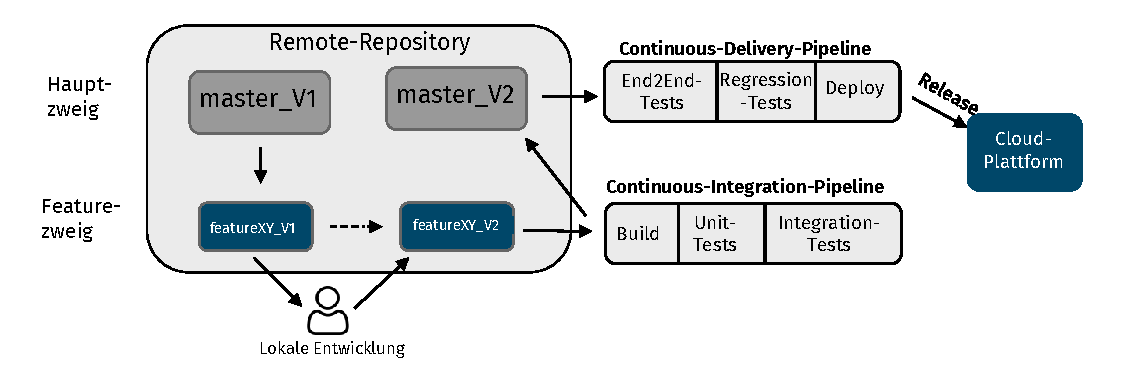
\includegraphics{VCS}}
		\caption[Integration der CI/CD-Pipeline mit dem Versionskontrollsystem]{Integration der CI/CD-Pipeline mit dem Versionskontrollsystem. Eigene Darstellung.}
		\label{fig:VCS}
	\end{figure}
\end{center}
\vspace*{-15mm}
Ein Repository stellt dabei einen zentralen Speicherort dar, welcher das Verfolgen sowie Überprüfen von Änderungen und ein paralleles bzw. konkurrierendes Arbeiten an einer gemeinsamen Codebasis ermöglicht \cite[31]{Loeliger.2012}. Der in dem Repository archivierte Hauptzweig (\textit{Master-Branch}) enthält eine aktuelle und funktionsfähige Version des Codes. Dieser mit verschiedenen Validierungsprozessen überprüfte Code stellt dabei die aktuelle in dem Produktionssystem laufende Anwendungsversion dar (s. Abb. \ref{fig:VCS}). Im Sinne der agilen Entwicklung werden große Softwareanforderungen (\textit{Epics}), in kleine Funktionalitäten (\textit{User Stories}) segmentiert, welche in separate Feature-Branches des Repositories ausgelagert werden. Diese sind unabhängige Kopien des Hauptzweiges, in welcher ein Entwickler Änderungen vornehmen kann, ohne Konflikte in der gemeinsamen Codebasis zu verursachen. Nach Fertigstellung der Funktionalitäten sollte der um die Features erweiterte Quellcode so schnell wie möglich in den Hauptzweig integriert werden \cite[169]{Loeliger.2012}. Die Einbindung des Feature-Branches in den Hauptzweig resultiert i.d.R. in einem unmittelbaren und automatisierten Start des \textbf{CI/CD-Pipeline-Prozesses}. Bei der CI/CD-Pipeline handelt es sich dabei um ein vom Repository unabhängiges Bereitstellungsautomatisierungs-Tool, welche auf einer virtuellen Maschine oder in einer containerisierten Computing-Umgebung betrieben wird \cite[Kap. 1.2]{Labouardy.2021}. Im ersten Schritt des Pipeline-Prozesses wird die Applikationen zu einem ausführbaren Programm kompiliert (\textit{Artefakt}) (\textit{Build}: s. Abb. \ref{fig:CICD_Cycle}). Dafür können je nach Programmiersprache verschiedene Build-Tools, wie NPM für JavaScript oder Make für \ac{MTA} verwendet werden \cite[Kap. 7.1]{Labouardy.2021}. Nach Ablauf der Build-Workflows erfolgt eine automatische Abwicklung des Validierungsprozesses (\textit{Smoke-Tests}).
\begin{center}
	\begin{figure}[H]
		\centering
		\scalebox{0.6}{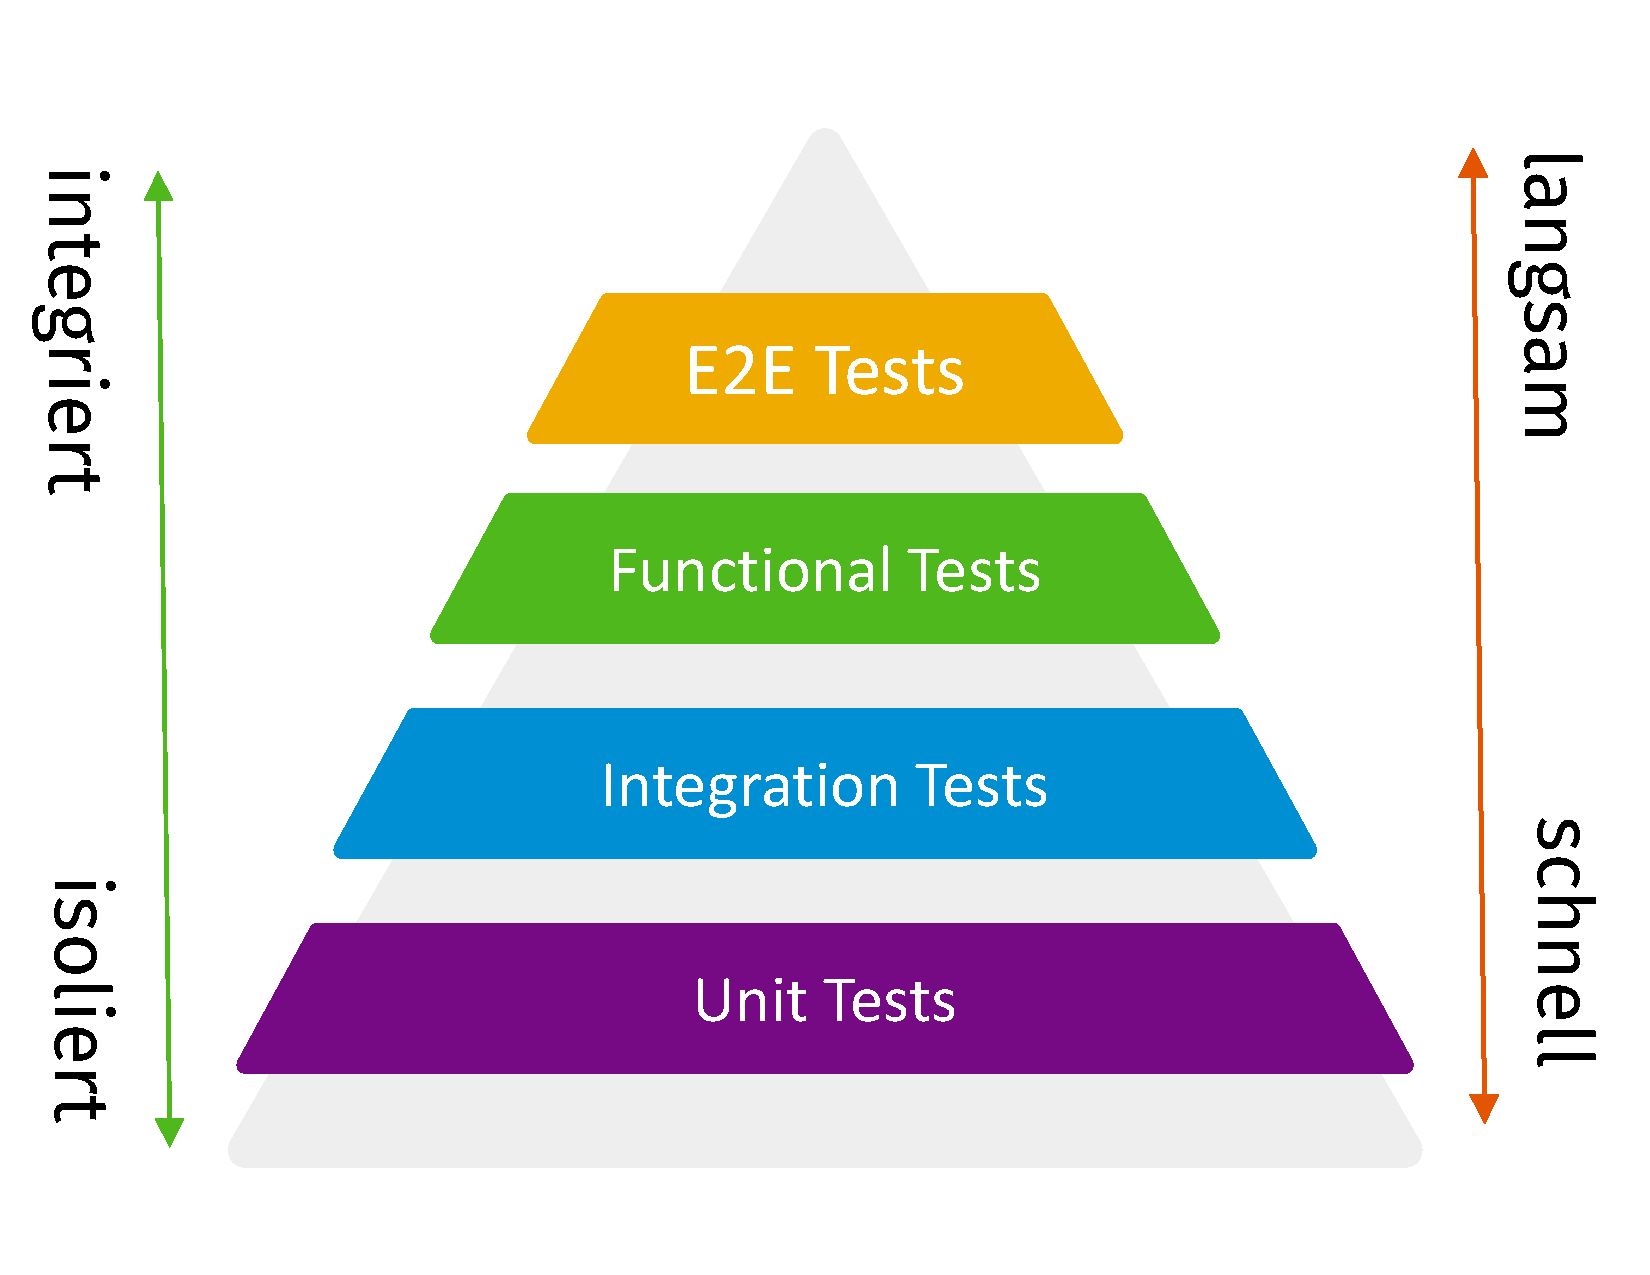
\includegraphics{Tests}}
		\caption[Hierarchische Darstellung von Softwaretests]{Hierarchische Darstellung von Softwaretests.\\ \hspace{0.5cm}In Anlehnung an Paspelava \cite{Exposit.2021}.}
		\label{fig:Tests}
	\end{figure}
\end{center}
\vspace*{-15mm}
Damit soll sichergestellt werden, dass zu jeder Zeit ein rudimentär getesteter Code bereitsteht und grundlegende Funktionalitäten sowie Schnittstellen erwartungsgemäß ausgeführt werden \cite[19]{Halstenberg.2020}. Die in diesem Schritt abgewickelten Tests leiten sich dabei aus der \textit{\ac{DoD}} ab. Die DoD ist eine in der Planungsphase festgelegte Anforderungsspezifikation, deren Erfüllung als notwendige Voraussetzung für den Abschluss eines Features gilt. Somit sind Entwickler dazu angehalten, für jedes implementierte Feature einen der DoD entsprechenden Tests zu entwerfen (\textit{Test Driven Development}). Der in dem CI-Prozess bereitgestellte Code wird dabei überwiegend anhand schnell durchführbarer Tests überprüft. Der Zweck dieser zügigen Validierungen liegt dabei insbesondere darin, dass Entwickler zeitnahes Feedback auf die Erweiterungen erhalten. So können Fehler und Konflikte so schnell wie möglich entdeckt und behoben werden, was die Entwicklung bei einer reibungslosen Auslieferung der IT-Services unterstützt. Die in der CI-Pipeline abgewickelten Validierungen umfassen i.d.R. \textit{Unit-} sowie \textit{Integration-Tests} \cite[Kap. 1.2]{Labouardy.2021}. Unit-Tests befinden sich dabei auf unterster Hierarchieebene der Test-Pyramide (s. Abb. \ref{fig:Tests}). Somit besitzen diese eine kurze Ausführungsdauer, werden jedoch ausschließlich in einer isolierten Testumgebung abgewickelt. Mit Unit-Tests wird die funktionale Korrektheit kleinster Einheiten, wie z.B. Methoden einer Klasse, über\-prüft. Der Zweck der Unit-Tests besteht dabei in einer von externen Einflüssen und Daten unabhängigen Überprüfung der einzelnen Komponenten \cite[Kap. 2]{Hambling.2015}. Um bei der Bereitstellung neuer Funktionalitäten ebenfalls das Zusammenspiel verschiedener Komponenten zu überprüfen, werden \textit{Integration-Tests} durchgeführt. Bei diesen Tests können Aspekte, wie der Austausch eines Nachrichtenmodells zweier Web-Services oder das Response-Objekt einer Datenbankabfrage untersucht werden \cite[Kap. 2]{Hambling.2015}. Im CI-Prozess werden i.d.R. auch einfache Code-Analysen durchgeführt. Diese sollen dem Entwickler eine schnelle Rückmeldung bezüglich Verletzung von Qualitätsstandards, potenziellen Schwachstellen sowie Leistungsproblemen liefern. Nachdem alle Tests erfolgreich absolviert wurden, kann sichergestellt werden, dass der neue Quellcode stabil, also funktionsfähig ist und keine Konflikte mit dem aktuellen Code des Hauptzweiges aufweist. Somit werden alle validierten Änderungen automatisch in dem Hauptzweig zusammengeführt. Mit diesem Prozessschritt beginnt der \textbf{Continuous-Delivery-Workflow (\acs{CD}-Workflow)}.  Während CI den Prozess der kontinuierlichen Integration des Quellcodes in das zentrale Repository verwaltet, steuert der CD-Workflow die Automatisierung der Anwendungsbereitstellung. Applikationen sollen somit ohne große Verzögerungen in die Produktivumgebung und somit zum Kunden ausgeliefert werden. Im Sinne des DevOps-Rahmenwerkes wird der CD-Prozess automatisch und unmittelbar nach Ablauf aller CI-Aktivitäten angestoßen. In der Praxis wird hierbei jedoch häufig ein manueller Schritt zwischengeschalten \cite[20]{Halstenberg.2020}. Damit soll sichergestellt werden, dass das Ausrollen der Anwendung erst nach Überprüfung und Genehmigung der Product Owner beginnt. Im ersten Schritt des CD-Prozesses wird das in die Produktivumgebung bereitzustellende Artefakt über die \textit{Deployment-Pipeline} in eine \textit{Staging-Area} geladen. Bei der Staging-Area handelt es sich dabei um ein System, welches zwischen Entwicklungs- und Produktivumgebung liegt. Die Staging-Systemkonfigurationen werden dabei so angelegt, dass diese der Produktionsumgebung möglichst ähnlich sind \cite[Kap. 1.3]{Labouardy.2021}. Neben Datenbanken werden hierbei ebenfalls Serverkonfigurationen, wie Firewall- oder Netzwerkeinstellungen von dem Produktivsystem übernommen. Somit soll sichergestellt werden, dass eine neue Anwendungsversion unter produktionsähnlichen Bedingungen getestet wird. Analog zum CI-Prozess werden innerhalb des CD-Workflows ebenfalls Unit- und Integration-Tests abgewickelt. Im Gegensatz zur CI-Pipeline werden dabei ebenfalls rechenintensive Tests automatisiert. Somit werden im CD-Prozess essenzielle, jedoch während des Entwicklungsworkflows zu aufwendige Validierungen durchgeführt \cite[20]{Halstenberg.2020}. Darüber hinaus werden in der Staging Area ebenfalls in der Test-Pyramide (s. Abb. \ref{fig:Tests}) höher positionierte, also rechenintensivere Tests ausgeführt \cite[Kap. 2]{Hambling.2015}. Dazu gehören \textit{\ac{E2E-Tests}}. Mit diesen soll sichergestellt werden, dass die Anforderungen aller Stakeholder erfüllt werden. Hierbei wird ein vollständiges Anwenderszenario von Anfang bis Ende getestet. Dabei wird i.d.R eine Benutzeroberfläche emuliert mit welcher etwa das Anmelden mit Benutzername, das Suchen eines Produktes und das Abschließen einer Bestellung validiert werden kann \cite{Bose.20230220}. Für kritische Systeme werden während des Delivery-Prozesses ebenfalls \textit{Regression-Tests} vorgenommen. Diese umfassen ein erneutes Testen bereits ausgelieferter Softwarekomponenten. Regression-Tests können dabei in Form von Unit-, Integration- sowie Functional-Tests ausgeführt werden. Somit soll sichergestellt werden, dass sich Quellcodeänderungen nicht negativ auf die stabile Anwendungsversion auswirkt. Auf oberster Ebene der Test-Pyramide befinden sich die \textit{Manual-Tests}. Dabei handelt es sich um von menschlichen Testern ausgeführte Validierungen, mit welchen Benutzerfreundlichkeit sowie Funktionalität anhand authentischer Anwenderszenarien gewährleistet werden soll. Da diese Tests nicht automatisiert durchgeführt werden können, muss der nächste Schritt der CD-Pipeline nach erfolgreicher Validierung manuell angestoßen werden. Im Anschluss werden i.d.R. verschiedene Codeanalysen abgewickelt. Hierbei werden Metriken, wie die prozentuale Testabdeckung oder Schwachstellen verwendeter Code-Patterns überprüft. Nach Durchführung der Codeanalysen wird das überprüfte Artefakt auf die Cloud-Plattform geladen (\textit{Deploy}: s. Abb. \ref{fig:CICD_Cycle}). Je nach Bereitstellungsstrategie (s. \ref{sec:Bereitstellungs_Strategien}), wird die Anwendung dann unmittelbar oder erst nach weiteren Überprüfungen für den Kunden zugänglich gemacht. Der letzte Schritt des CD-Workflows umfasst die Laufzeitüberwachung der inbetriebgenommenen Anwendung (\textit{Monitoring}: s. Abb. \ref{fig:CICD_Cycle}). Diese wird i.d.R. durch ein unabhängiges Überwachungssystem und nicht von dem Pipeline-Tool selbst abgewickelt. Dabei können z.B. Dashboards zur Analyse der Build-, Test- und Deployment-Prozesse visualisiert werden. Darüber hinaus umfasst dieses Tool essenzielle Überwachungselemente zum \textit{Infrastruktur-}, \textit{Plattform-} sowie \textit{Anwendungs-Monitoring}. Beim Infrastruktur-Monitoring werden Metriken wie CPU-, Speicher- und Netzwerklast der Server bzw. Datenbanken untersucht. Das Plattform-Monitoring setzt dabei eine Ebene höher an und validiert, dass Komponenten wie Datenbanken, virtuelle Netze bzw. Middlewares ordnungsgemäß durchgeführt werden. Das Anwendungs-Monitoring umfasst die Überwachung der Funktionalitäten und der Applikation selbst \cite[21]{Halstenberg.2020}.\\ 
Zur Automatisierung der CI/CD-Prozesse werden von der SAP i.d.R. drei verschiedene Tools vorgeschlagen. Eine unmittelbare von der SAP bereitgestellte Lösung ist das \textit{\ac{SAP CI/CD}}. Das SAP CI/CD ist eine auf der SAP BTP betriebene SaaS-Lösung, mit welcher vordefinierte Pipeline-Templates konfiguriert und ausgeführt werden können. Dieses Tool ist insbesondere mit SAP-Standardtechnologien, wie den Programmierframeworks SAP UI5 und SAP CAP Node sowie der Laufzeitumgebung Cloud-Foundry kompatibel \cite{.20230405}. Eine weitere bei der SAP empfohlene CI/CD-Alternative ist das Open-Source-Tool \textit{Jenkins}. Im Gegensatz zum templatebasierten SAP CI/CD, muss der Bereitstellungsworkflow bei Jenkins mit der Programmiersprache Groovy implementiert werden. Weiterhin wird Jenkins nicht unmittelbar auf der SAP BTP betrieben, sondern muss auf einem eigenen Server (On-Premise) verwaltet werden \cite[Kap. 2]{Labouardy.2021}. Um die Bereitstellung von SAP-spezifischen Technologien zu optimieren, wurde die Programmbibliothek \textit{Project Piper} verföffentlicht. In Project Piper werden vorimplementierte Pipeline-Schritte und die dafür benötigten Treiber gebündelt. Im Gegensantz zum SAP CI/CD sind diese jeodoch hoch konfigierbaren.
Ein externes ebenfalls von der SAP vorgeschlagenes CI/CD-Werkzeug ist \textit{Azure Pipelines}. Azure Pipelines ist ein von Microsoft entwickeltes Tools, welches umfassende Integrationsmöglichkeiten zu anderen Microsoft-Diensten wie die Azure-Cloud-Platform oder Microsoft Visual Studio Code bietet. Zur Implementierung des CI/CD-Workflows SAP-spezifischer Technologien wird für Azure Pipelines ebenfalls die Programmbibliothek Project-Piper verwendet.
\subsubsection{Strategien zur Bereitstellung von Neuentwicklungen}
\label{sec:Bereitstellungs_Strategien}
Nachdem das Artefakt auf einer virtuellen Maschine bzw. containerisierten Cloud-Instanz installiert und gestartet wurde, erfolgt die Inbetriebnahme der neuen Anwendungsversion je nach Bereitstellungsstrategie unmittelbar oder erst nach weiteren Validierungen. Anhand der Bereitstellungsstrategie wird festgelegt, mit welcher Methode und zu welchem Zeitpunkt Nutzeranfragen von der aktuellen auf die neue Anwendungsinstanz umgeleitet werden (s. Abb. \ref{fig:DS}).
Eine häufig verwendete Deployment-Strategie ist dabei das \textit{Blue/Green-Deployment}. Hierbei wird neben der stabilen aktuellen Anwendung (\textit{Blaue Version}) ebenfalls eine Instanz des neuen IT-Services (\textit{Grüne Version}) in dem Produktionssystem betrieben. Das impliziert, dass der alte IT-Service nicht unmittelbar, sondern erst nach verschiedenen im Produktionssystem durchgeführten Validierungen durch die aktualisierte Version ersetzt wird. Ein Vorteil dieser Vorgehensweise besteht darin, dass die neue Version nicht in einer Staging-Area, sondern unmittelbar unter produktionsähnlichen Bedingungen geprüft werden kann \cite{Ugochi.20220503}. Ein zusätzlicher positiver Effekt entsteht in Zusammenhang mit der durch die Aktualisierung verursachten Ausfallzeit. Im herkömmlichen Bereitstellungsverfahren wird die alte Anwendungsversion gestoppt, der neue Service installiert und dann gestartet. Dadurch kann der Dienst erst nach erfolgreicher Inbetriebnahme der neuen Instanz wiederverwendet werden, was i.d.R. zu längeren Ausfallszeiten führt. Dies kann jedoch mithilfe des Blue/Green-Deployments vermieden werden. Hierbei wird die neue Anwendungsversion  auf einer separaten Instanz installiert. Sobald die neue Version erfolgreich gestartet ist, kann der Datenverkehr unmittelbar auf diese umgeleitet werden. Somit können längere Ausfallszeiten umgangen werden. 
\begin{center}
	\begin{figure}[H]
		\centering
		\scalebox{0.4}{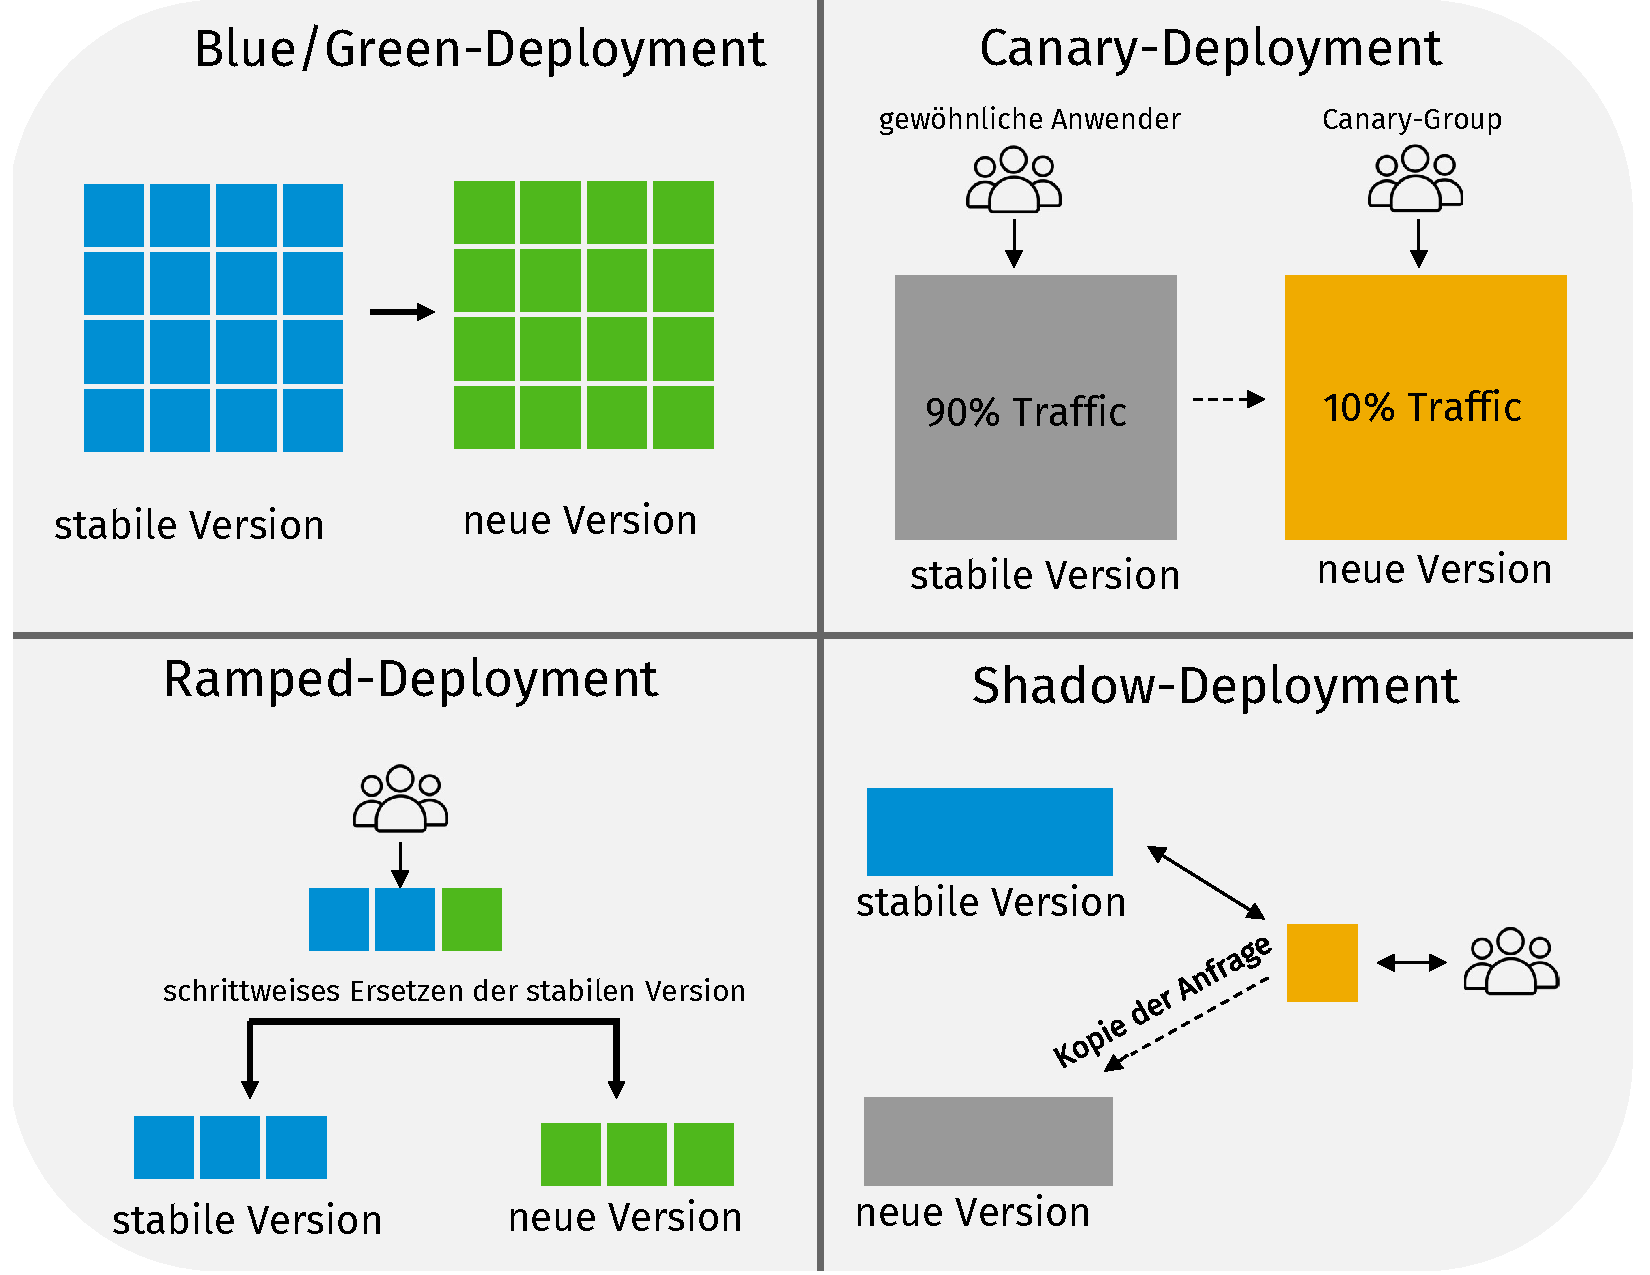
\includegraphics{Deployment_Strategies}}
		\caption[Strategien zur Bereitstellung von Software]{Strategien zur Bereitstellung von Software.\\ In Anlehnung an Ugochi \cite{Ugochi.20220503}.}
		\label{fig:DS}
	\end{figure}
\end{center}
\vspace*{-15mm}
Im Gegensatz dazu wird im Blue-Green-Deployment die neue Anwendung auf einer separaten Instanz installiert. Sobald die neue Version erfolgreich gestartet wurde, kann der Datenverkehr unmittelbar auf diese umgeleitet werden. Im Vergleich zum Blue/Green-Deployment, bei welchem eine neue Version simultan für die gesamte Nutzerbasis zur Verfügung gestellt wird, gewährleistet das \textit{Canary-Deployment} eine restriktivere Nutzlastumleitung. Hierfür wird die neue Anwendungsversion vorerst einer überschaubaren Nutzeranzahl (\textit{Canary-Gruppe}) bereitgestellt. Dabei sollte die zusammengestellte Canary-Gruppe die Gesamtnutzerbasis möglichst gut repräsentieren. Anhand des Canary-Traffics soll der fehlerfreie Betrieb neuer Anwendungen überprüft und ggf. Anpassungen vorgenommen werden. Bevor die neue Anwendungsversion der gesamten Nutzerbasis zur Verfügung gestellt wird, kann diese sukzessive und schrittweise ausgerollt werden \cite{Ugochi.20220503}. Eine aufwendigere, jedoch risikoärmere Bereitstellungsstrategie stellt das \textit{Shadow-Deployment} dar. Dabei wird neben der Instanz der aktuellen Version ebenfalls ein sog. \textit{Shadow-Model} auf der Infrastruktur betrieben. Das Shadow-Model verwaltet die neue Version der Anwendung, kann jedoch nicht unmittelbar von den Nutzern aufgerufen werden. Diese Instanz stellt ein hinter der stabilen Version gelagertes Schattenmodell dar. Benutzeranfragen werden von dem Load-Balancer stets auf die aktuelle Version der Instanz weitergeleitet, verarbeitet und beantwortet. Gleichzeitig wird eine Kopie dieser Anfrage an das Shadow-Model weitergeleitet und von diesem prozessiert. Die Shadow-Modell-Verarbeitung des in der Produktionsumgebung abgewickelten Netzwerkverkehrs ermöglicht den Entwicklern somit eine anwendungsbezogene Überprüfung entwickelter Features \cite{Ugochi.20220503}. Ein weiteres Bereitstellungskonzept ist das \textit{Multi-Cloud-Deployment}. Dieses wird verwendet, um ERP-Dienste in einer verteilten Computing-Umgebung auszuführen. Dabei werden die Anwendungen eines Unternehmens i.d.R. auf verschiedenen Cloud-Plattformen bereitgestellt. Der Vorteil dieser Bereitstellungsstrategie besteht darin, dass durch diese Diversifizierung verschiedene Technologien verwendet und somit eine höhere Skalierbarkeit, Verfügbarkeit und Performance der Anwendung erreicht werden kann.